\documentclass[11pt,a4paper]{article}
\usepackage{fullpage}
\usepackage{tgadventor}
\usepackage[T1]{fontenc}
\newcommand{\hsp}{\hspace{20pt}}
\newcommand{\HRule}{\rule{\linewidth}{0.5mm}}
\usepackage{float}
\usepackage{amsmath}
\usepackage{caption}
\usepackage{subcaption}
\usepackage{graphicx}
\usepackage{xcolor}
\usepackage{hyperref}
\definecolor{darkblue}{RGB}{14,43,88}

\makeatletter
\newcommand{\authors}{%
  \setlength\arrayrulewidth{2pt}
  \begin{tabular}{l|l}
  \@authorsi
}
\newcommand\@authorsi{\@ifnextchar\stopauthors{\@authorsend}{\@authorsii}}
\newcommand\@authorsii[2]{%
  \\
  \textbf{\Large #1} &  \textbf{\Large #2}
  \\
  \@authorsi % restart the recursion
}
\newcommand\@authorsend[1]{
  \end{tabular}}
\makeatother

%%%%%%%%%%%%%%%%%%%%%%%%%%%%%%%%%%%%%%%%%%%%%%%%%%%
%%%%%%%%%%%% Define following Variables %%%%%%%%%%%
%%%%%%%%%%%%%%%%%%%%%%%%%%%%%%%%%%%%%%%%%%%%%%%%%%%
\def \classSigle{LMAPR2451}
\def \className{Atomistic and nanoscopic simulations}
\def \workName{Study of pyrite / FeS$_\text{2}$ and its optical properties}
\def \professors{Professors Jean-Christophe Charlier, Xavier Gonze \& Gian-Marco Rignanese\\Mentors : Alexandre Cloots \& Ionel-Bogdan Guster}
\def \academicYear{2020-2021}
\def \abstractText{This report aims to investigate the optical properties of pyrite (FeS$_\text{2}$). To do so, \textit{ab initio} computations are first performed on a 6-atoms unit cell. The convergence with respect to several structural parameters is also studied. The optical properties are then analyzed in the light of the obtained results. Finally, a comparison is made with the already existing documentation, and a discussion about the quality of the simulation is made.}
%%%%%%%%%%%%%%%%%%%%%%%%%%%%%%%%%%%%%%%%%%%%%%%%%%%
%%%%%%%%%%%%%%%%%%%%%%%%%%%%%%%%%%%%%%%%%%%%%%%%%%%
%%%%%%%%%%%%%%%%%%%%%%%%%%%%%%%%%%%%%%%%%%%%%%%%%%%

\begin{document}
\begin{titlepage}
\begingroup
\fontfamily{\sfdefault}
  \begin{flushleft}  
  \begin{minipage}{0.55\textwidth}
  
\includegraphics[width=\textwidth]{images/epl2.png}
  \end{minipage}
  \end{flushleft}
  \centering
  \textcolor{darkblue}{{\huge \textbf{\classSigle \\[0.1cm] \className}}}
  \vfill
  \textcolor{darkblue}{
  \hrule height 0.1cm
  \hspace{1cm}\\[0.3cm]
  {\Huge \textbf{\workName}}\\[0.5cm]
  \hrule height 0.1cm
  \hspace{1cm}\\[0.3cm]
  {\Large\textbf{\professors}}}
  \vfill
  \begin{minipage}[c]{\textwidth}
  \centering
  \textcolor{darkblue}{
  \authors
  %%%%%%%%%%%%%%%%%%%%%%%%%%%%%%%%%%%%%%%%%%%%%%%%%
  %%%%Mettre un auteur par ligne sous le format%%%%
  %%%%%%%%%%%%%%%%{Nom Prénom}{NOMA}%%%%%%%%%%%%%%%
  %%%%%%%%%%%%%%%%%%%%%%%%%%%%%%%%%%%%%%%%%%%%%%%%%
  {Anatole Moureaux}{54731700}
  %%%%%%%%%%%%%%%%%%%%%%%%%%%%%%%%%%%%%%%%%%%%%%%%%
  %%%%%%%%%%%%%%%%%%%%%%%%%%%%%%%%%%%%%%%%%%%%%%%%%
  %%%%%%%%%%%%%%%%%%%%%%%%%%%%%%%%%%%%%%%%%%%%%%%%%
  \stopauthors}
  \end{minipage}
  \vfill
  \noindent\fbox{%
    \parbox{1\textwidth}{%
        \centering
         \textcolor{darkblue}{\textbf{\abstractText}}%
        }
    }
  \vfill
  \begin{center}
  \textcolor{darkblue}{\textbf{\Large \academicYear}}
  \end{center}
\endgroup
\end{titlepage}
\tableofcontents
\newpage
\section{Introduction}
\subsection{Motivations}
Pyrite (FeS$_2$) (\autoref{fig:minerai}) is an interesting semiconducting material. Indeed, it can be used in numerous domains, from mechanical applications, where it is appreciated for its toughness and abrasiveness, to optical applications, where it can be used as an high-energy light absorber \cite{pyriteApps}. As pyrite is very abundant, it can become a material of choice in the industry if correct and valuable uses of the latter could be elaborated.

One of the promising potential application of pyrite is its integration into solar panels. Indeed, pyrite thin films could be good alternatives to the conventional silicon based solar cells, which are more economically and ecologically costly. However, the performances of the material must be similar to materials already used for solar cells, in order to make it truly competitive \cite{pyriteSolarCells}.It is thus important to assess the different optical characteristics that pyrite is able to present. 

Solar cells are not a new concept. However, it might be interesting to recall some of the main features of thoses devices. It consist of photoelectric components able to convert the energy of the (solar) light into electricity though the \textit{photovoltaic effect}. More precisely, a solar cell is composed of a \textit{pn}-junction diode, usually made of silicon. When the depletion region of the junction is hit by solar photons, an electron is delivered in the $n$-layer and a hole is delivered in the $p$-layer (\autoref{fig:pnjunction}). By doing so on a large scale, the \textit{pn}-junction is able to generate a voltage of about $0.5$ [V], if the $n$-doped layer is sufficiently thin (to make the photons reach the depletion region as easily as possible). A solar panel is composed of several solar cells in series, in order to add up the voltage generated by each cell. The best materials for solar cells-related applications are the materials showing :
\begin{itemize}
\item a semiconducting behavior
\item a high optical absorption coefficient
\item a high electrical conductivity
\item an abundant presence in the Earth's crust.\cite{solarCell}
\end{itemize}
\begin{figure}[H]
\centering
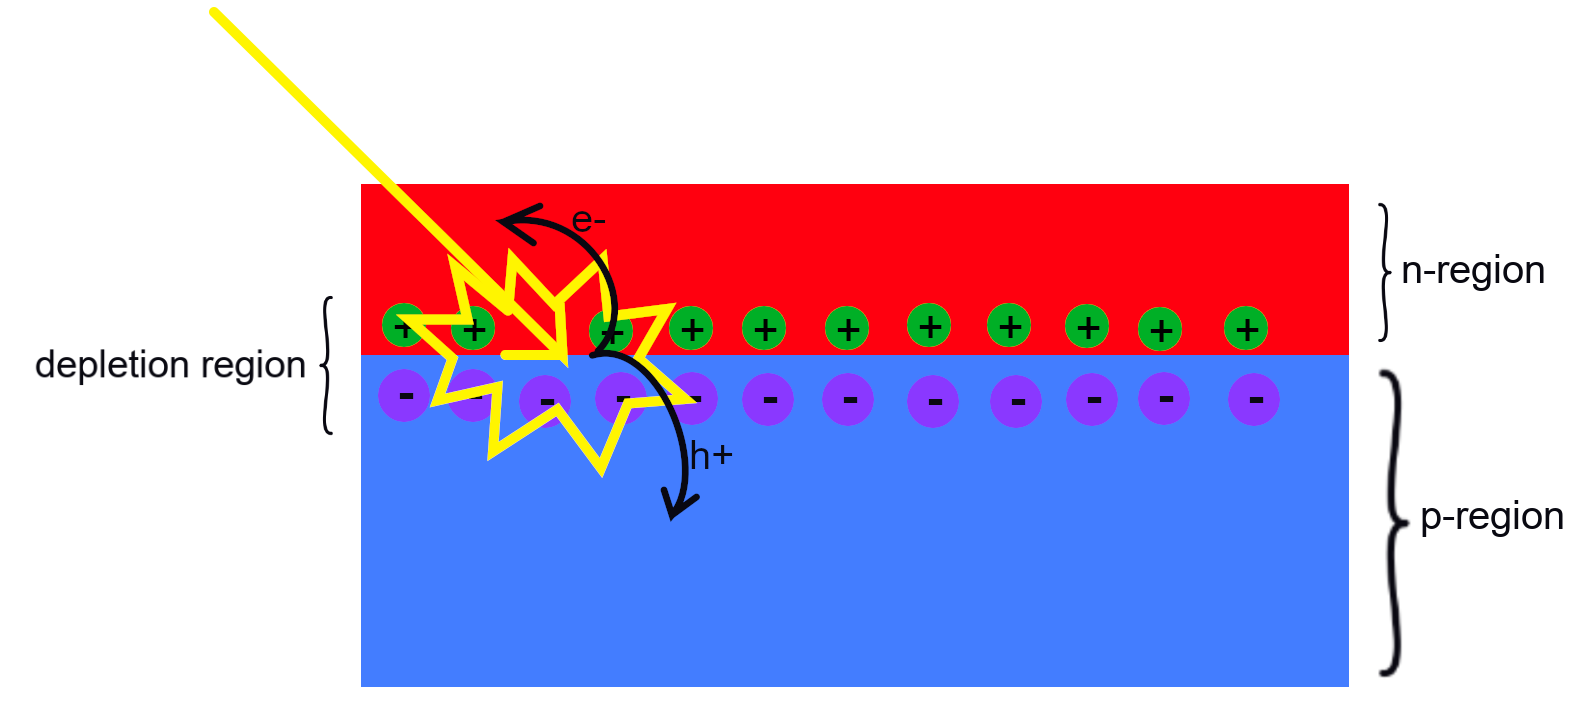
\includegraphics[width=0.8\textwidth]{images/pnjunction.png}
\caption{Simplified view of the photovoltaic effect. When a photon hits an atom in the depletion region, an electron is released in the $n$-region and a hole is released in the $p$-region, creating a voltage when done multiple times.}
\label{fig:pnjunction}
\end{figure}
Even if bulk pyrite shows a $n$-type behavior, pyrite thin-films show high levels of $p$-type doping. Only the deposition of a thin layer of $n$-type semiconductor on the pyrite film is needed to form a $pn$-heterojunction. Furthermore, the pyrite has a strong absorption coefficient. It thus allows to decrease the thickness of the pyrite film, which is helpful to improve the performances of the $pn$-junction, and hence, of the solar cell \cite{thinFilms}. Plus, it is abundant in the soil. Pyrite thus seems to be a material of choice for solar cells-related applications.

However, serious limitations prevent pyrite to be highly performant in solar cells-based applications. Indeed, a very poor solar energy conversion efficiency is observed when assessing the performances of pyrite solar cells. That low efficiency is presumably due to low a photovoltage generation. The sources of that low photovoltage is a highly debated topic in among the scientific community. Several sources have been proposed over the years : detrimental S vacancies (although stœchimetric pyrite shows the same low photovoltage), detrimental impurities or even lattice defects \cite{limitations}. No consensus has been found nowadays. But as pyrite could be a game-changer in the solar cell industry if its efficiency was improved, it is worth to look a little closer to the optical properties of the material.

In the following report, the properties of the \textsc{Pnnm} FeS$_2$ will be studied using the \texttt{Abinit} package. First, the unit cell and its structural parameters will be described, based on the Materials Project documentation\footnote{\url{https://materialsproject.org/materials/mp-1522/}}. Then, the representation of the crystal in \texttt{Abinit} will be presented (thus describing the main parameters of the \texttt{.abi} files to be used). Secondly, the pseudopotential and the approximation used in the first place will be discussed. Then, convergence studies based on the energy cut-off (\texttt{ecut}) and the number of $k$-points (\texttt{ngkpt}) will be performed. When a proper (\texttt{ecut},\texttt{ngkpt}) will have been determined, a discussion about the pseudopotential and the approximation will be held, and possible alternatives will be presented. Finally, additional \texttt{Abinit} computations will be made, and the optical properties will be studied through other characteristics of the material. To conclude, the performances of pyrite in solar cells-based applications will be discussed.
\subsection{Pyrite : Overview and \texttt{Abinit} representation}
The pyrite (FeS$_2$) primitive cell contains 2 Fe atoms and 4 S atoms, and is part of the orthorombic system (\autoref{fig:primitiveCell}). The space group is \textsc{Pnnm}[58] in the Hermann-Mauguin notation. 

Furthermore, it is a semiconductor. The energy of the indirect bandgap $\left(\begin{pmatrix}
0 & 0.4 & 0
\end{pmatrix}-\textsc{U}\right)$ is about 0.978 [eV]\cite{MaterialsProject}.

Finally, the primitive cell will be represented as follow in \texttt{Abinit} input files :
\begin{center}
\begin{tabular}{lll}
\texttt{acell} & \texttt{3.390} \texttt{4.438} \texttt{5.411} \texttt{Angstr} & \texttt{\# the lattice vectors scaling}\\
\texttt{ntypat} & \texttt{2} & \texttt{\# there are two types of atoms in the}\\
&&\texttt{\#\space\space\space\space primitive cell : Fe and S}\\
\texttt{znucl} & \texttt{26 16}& \texttt{\# Fe has 26 electrons and S has 16}\\
\texttt{natom} & \texttt{6} & \texttt{\# there are 6 atoms in the primitive cell}\\
\texttt{typat} & \texttt{1 1 2 2 2 2}&\texttt{\# 2 Fe atoms and 4 S atoms}\\
\texttt{xred} & \texttt{0\space\space\space\space\space\space 0\space\space\space\space\space\space 0} & \texttt{\# position of the first Fe atom in reduced coordinates}\\
& \texttt{0.5\space\space\space\space 0.5\space\space\space\space0.5} & \texttt{\# position of the second Fe atom}\\
& \texttt{0\space\space\space\space\space\space 0.206\space\space 0.3753} & \texttt{\# position of the first S atom}\\
& \texttt{0\space\space\space\space\space\space 0.794\space\space 0.6247} & \texttt{\# position of the second S atom}\\
& \texttt{0.5\space\space\space\space 0.294\space\space 0.8753} & \texttt{\# position of the third S atom}\\
& \texttt{0.5\space\space\space\space 0.706\space\space 0.1247} & \texttt{\# position of the fourth S atom}\\
\end{tabular}
\end{center} 
The data also comes from \cite{MaterialsProject}.
\begin{figure}[H]
\centering
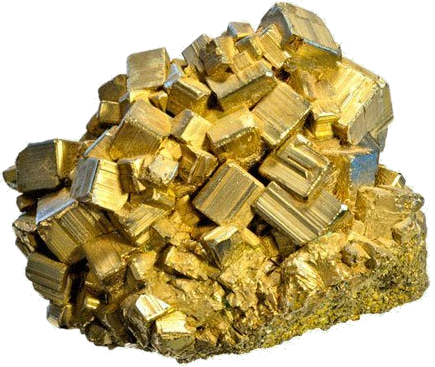
\includegraphics[width=0.6\textwidth]{images/pyrite}
\caption{Extracted form (ore) of pyrite.\\
"Pierre Pyrite", France Minéraux, 2021.}
\label{fig:minerai}
\end{figure}
\begin{figure}[H]
\centering
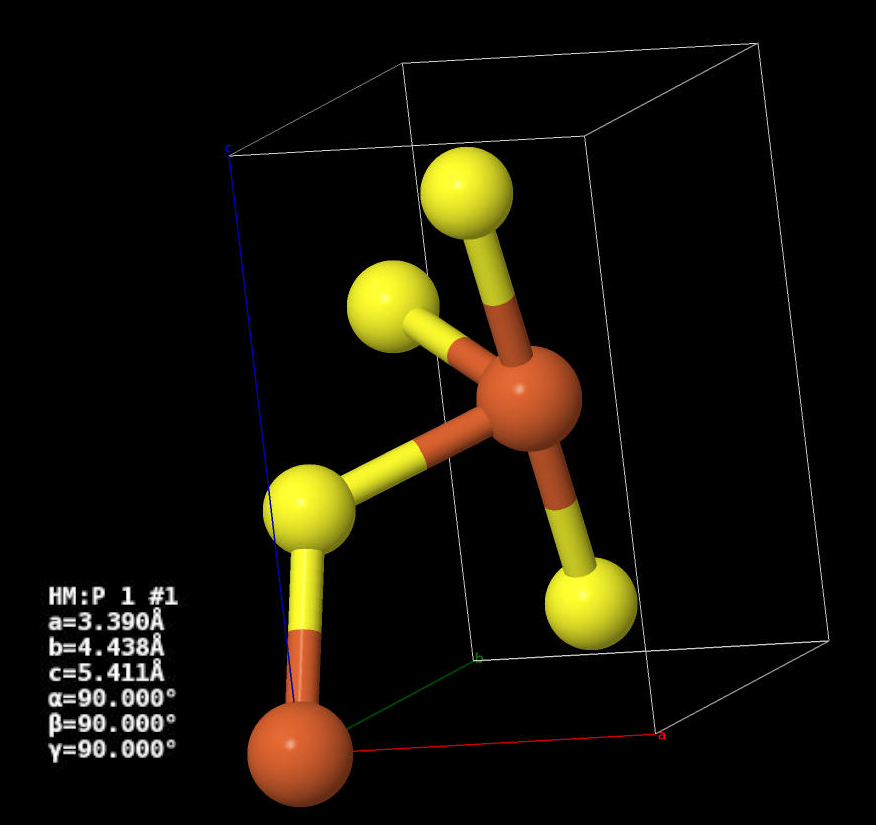
\includegraphics[width=0.61\textwidth]{images/primitiveCell}
\caption{Primitive cell of FeS$_2$.\\Materials Project (mp-1522), Jmol}
\label{fig:primitiveCell}
\end{figure}
\newpage
\section{Convergence studies and pseudopotentials}
In \texttt{Abinit} computations, convergence studies are very important, as it help to make sure that some of the chosen parameters, like the cut-off energy (\texttt{ecut}) or the number of $k$-points in the cell (determined by the sampling of the Brillouin zone \texttt{ngkpt}), allow the most accurate results as possible. To do such analysis, the same computations are done with a dataset concerning the parameter of interest, with an increasing accuracy of the environment. The evolution of some resulting variables, like the total energy of the unit cell (\texttt{etotal}), indicates when the parameters of interest allow a sufficiently accurate simulation.

In the following subsections, the convergence studies with respect to \texttt{ecut} and \texttt{ngkpt} will be performed. One could also choose to study the convergence of the simulation with respect to the scaling of the lattice parameters (\texttt{acell}). However, the complexity of this kind of study increases pretty fast with the number of atoms in the unit cell, and as pretty accurate values were found on the Materials Project, this study won't be performed here. It is still possible to optimize the shape and the volume of the unit cell when the final \texttt{ecut} and \texttt{ngkpt} are chosen, in order to get the most accurate future computations as possible.
\subsection{Additional parameters}
To begin, we will use the \textit{Local spin Density Approximation} (LDA) functional. Indeed, it is widely used and works well in many simulations. The pseudopotentials that will be used are retrieved from the pseudodojo \cite{PseudoDojo}. Two pseudopotentials are used : the NC SR (ONCVPSP v0.4.1) LDA standard pseudopotential relative to Fe, and the same one but relative to S (both in psp8 format).

It is also important to properly define the parameters ruling the SCF procedure. The most important one is \texttt{nstep}, defining the number of SCF cycles. It is set to \texttt{50} in the first place, but can be easily increased if it is not sufficient. \texttt{toldfe} is set to \texttt{1.0d-10}, ensuring a pretty accurate convergence with respect to the total energy. \texttt{toldfe} is chosen as the structural relaxation is not performed yet (in that case, \texttt{toldff} is preferably used). Although it is not mandatory, the SCF procedure can be preconditioned by specifying the macroscopic dielectric constant (\texttt{diemac}). It is used to speed up the SCF procedure. A value of \texttt{24} is chosen, accordingly to \cite{MaterialsProject}. 

Finally, the parameters of the $k$-points grid must be specified. \texttt{kptopt} is set to \texttt{1} in order to take advantage of the symmetry of the unit cell. 
By setting \texttt{prtkpt} to \texttt{1}, \texttt{Abinit} will generate a set of $k$-point grids, that will be helpful to optimize further computations and convergence studies.
\begin{center}
\begin{tabular}{lll}
\texttt{pseudos} & \multicolumn{2}{l}{\texttt{"pdj\_nc\_sr\_041\_lda\_standard\_psp8/Fe.psp8, pdj\_nc\_sr\_041\_lda\_standard\_psp8/S.psp8"}}\\
&&\\
\multicolumn{3}{l}{\texttt{\# parameters of the SCF procedure : }}\\
\texttt{nstep} & \texttt{50} &\texttt{\# maximal number of SCF cycles}\\
\texttt{toldfe} & \texttt{1.0d-10} &\texttt{\# SCF procedure will stop when the difference of total energy}\\
&&\texttt{\#\space\space\space\space between two iterations will be lower than toldfe Hartree}\\
\texttt{diemac} &\texttt{24.0} & \texttt{\# preconditioning of the SCF procedure.}\\
&&\\
\multicolumn{3}{l}{\texttt{\# parameters of the k-points grid : }}\\
\texttt{kptopt} & \texttt{1} &\\
\texttt{prtkpt} & \texttt{1} 
\end{tabular}
\end{center}
\subsection{Determination of the optimal $k$-points grid}
The first simulation will be used to generate $k$-points grids and the corresponding shifts (\texttt{shiftk}). \texttt{Abinit} was run with the input file \texttt{1522\_1\_kpointsgrids.abi} (\autoref{Abi1}), performing the analysis of a series of 70 different $k$-grids. The lists were provided with the corresponding \texttt{kptrlatt}, \texttt{shiftk}, \texttt{kptrlen} and \texttt{nkpt} parameters. An additional list containing the best $k$-grids was also provided, helping to have a better idea of the $k$-points distribution in the irreducible Brillouin zone.

To conclude, the default Monkhorst-Pack grids will be used, by using
\begin{center}
\begin{tabular}{lll}
\texttt{ngkpt} & \texttt{4 4 4}&\\
\texttt{nshiftk} & \texttt{1} &\\
\texttt{shiftk} &\texttt{0.5 0.5 0.5}
\end{tabular}
\end{center}
\subsection{Convergence with respect to \texttt{ecut}}
The study of the convergence of the simulation was performed by running \texttt{Abinit} with the input file \texttt{1522\_1\_ecutConv.abi} (\autoref{Abi2}).
The total energy of the unit cell \texttt{etotali} for each \texttt{ecut} $i$ is then plotted versus \texttt{ecut} (which spans from $10$ [Ha] to $58.33$ [Ha]) (\autoref{fig:ecutConv}, upper plot). The total energy per atom can also be plotted (\autoref{fig:ecutConv}, lower plot). Upper and lower bounds of $\pm 0.5$ [mHa] are set around the last obtained value. It allows to determine the first \texttt{ecut} for which the convergence is reasonable. In the present case, \texttt{ecut} = \texttt{40} [Ha].
\begin{figure}[H]
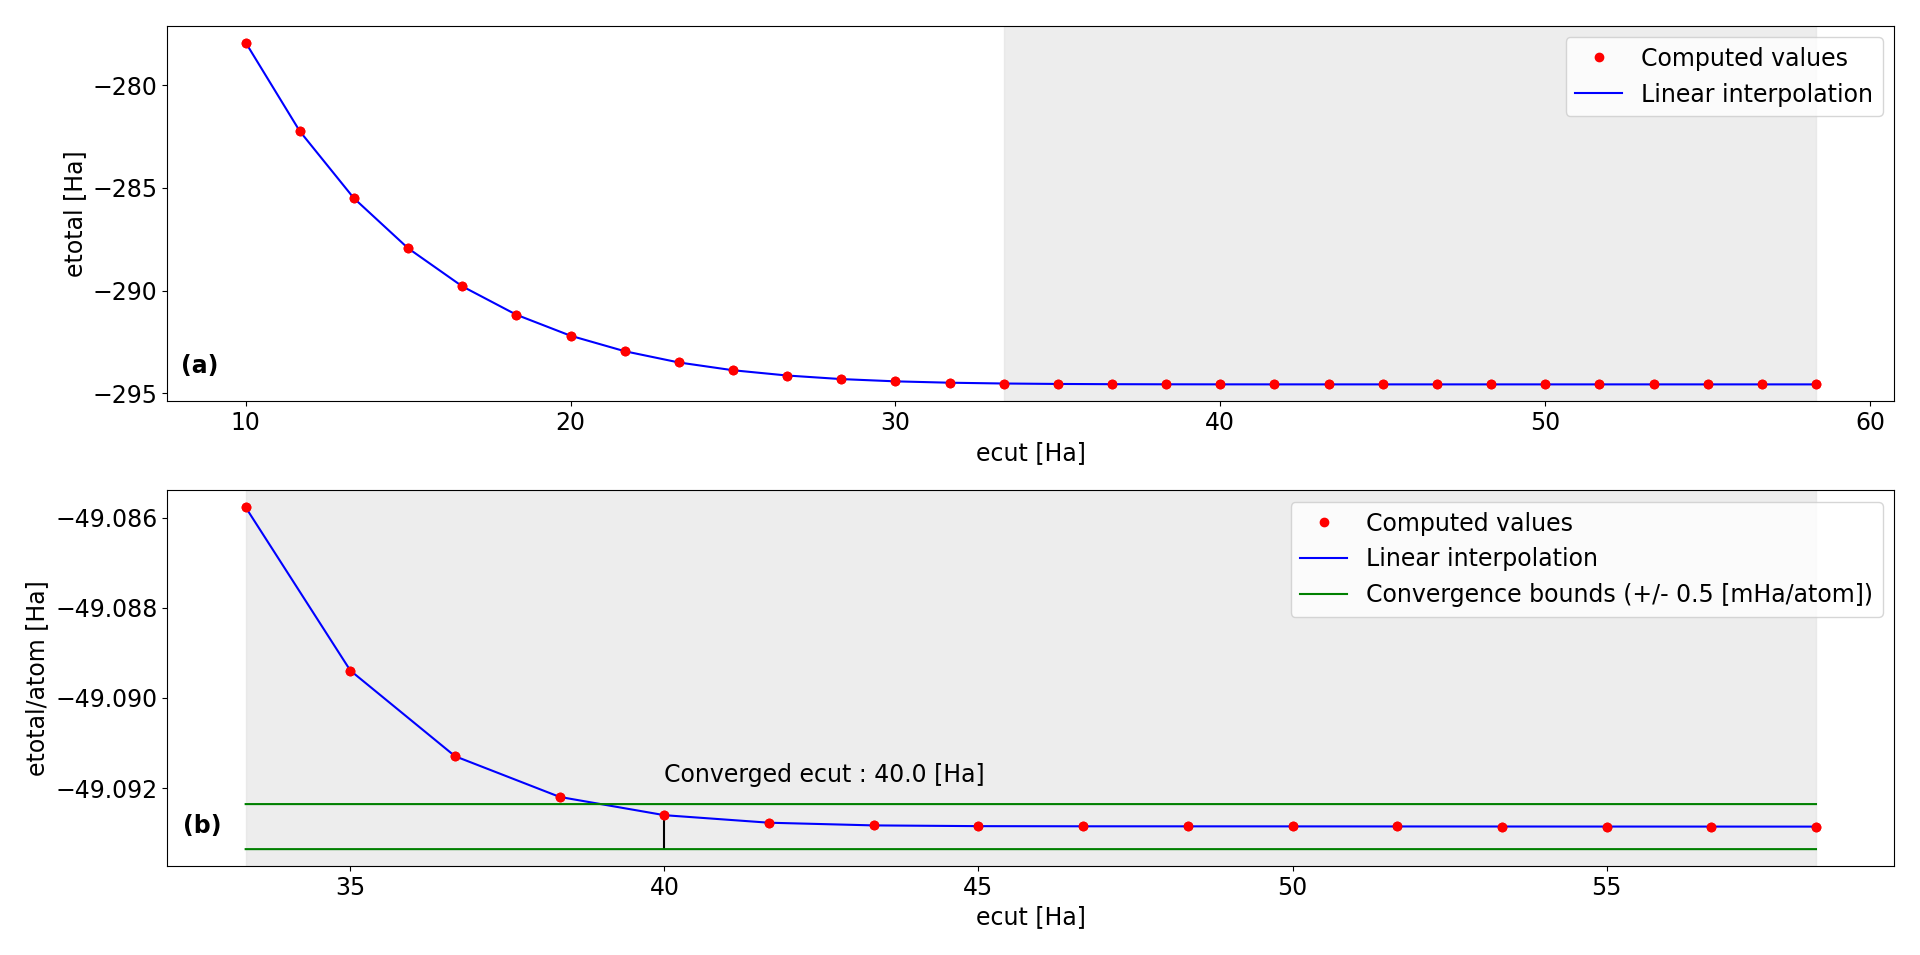
\includegraphics[width=\textwidth]{images/ecutConv}
\caption{Total energy (upper) and total energy per atom (lower) with respect to the cut-off energy.}
\label{fig:ecutConv}
\end{figure}

\subsection{Convergence with respect to \texttt{ngkpt}}
Alternatively, the same kind of study is done for the number of $k$-points in the lattice. \texttt{Abinit} is run with the input file \texttt{1522\_1\_nkpConv.abi}(\textcolor{red}{mettre le bon ecut}) (\autoref{Abi3}). The total energy and the energy per atom can be plotted versus the \texttt{ngkpt} parameter.

\textcolor{blue}{
\textbackslash\textbackslash TODO\\
- Summarize the (ecut,ngkpt) that will be used for the further computations}
\subsection{Determination of the lattice parameters (relaxation)}
\textcolor{blue}{
\textbackslash\textbackslash TODO\\
- With the final (ecut,ngkpt), optimize acell}
\subsection{Pseudopotentials}
\textcolor{blue}{
\textbackslash\textbackslash TODO\\
- Describe (an)other(s) pseudopotential(s), explain the pros and cons => choose a better pseudopotential if needed}
\newpage
\section{Optical properties}
\textcolor{blue}{
\textbackslash\textbackslash TODO\\
- Compute the electronic band structure\\
- compute the phonon dispersion\\
- Implications for a thin film used in a solar cell}
\newpage
\section{Comparison with the litterature}
\textcolor{blue}{
\textbackslash\textbackslash TODO\\
- Compare with the material project + other sources if needed\\
- Discuss the differences and the similitudes}
\newpage
\section{Conclusion}
\textcolor{blue}{
\textbackslash\textbackslash TODO\\
- Summary of the study
- What has been learned ? \\
- What implications in real life applications ?\\
- What further studies could be done ?}
\newpage
\begin{thebibliography}{00}
\bibitem{pyriteApps} "Pyrite de fer - Utilisations et applications | African Pegmatite", African Pegmatite, 2021. [Online]. Available: \url{https://mineralmilling.com/fr/pyrite-de-fer-utilisations-et-applications/}. [Accessed: 04- Apr- 2021].
\bibitem{pyriteSolarCells} M. Hutchins, "A long way to go for iron pyrite solar cells", pv magazine International, 2021. [Online]. Available: \url{https://www.pv-magazine.com/2020/06/15/a-long-way-to-go-for-iron-pyrite-solar-cells/}. [Accessed: 04- Apr- 2021].
\bibitem{solarCell} "Solar Cell: Working Principle \& Construction (Diagrams Included)", Electrical4U, 2021. [Online]. Available: \url{https://www.electrical4u.com/solar-cell/}. [Accessed: 05- Apr- 2021].
\bibitem{thinFilms} M. Limpinsel, "Iron Pyrite Absorbers for Solar Photovoltaic Energy Conversion", University of California, 2015. Available: \url{https://escholarship.org/uc/item/8042w4kd}. [Accessed 5 April 2021].
\bibitem{limitations} M. Rahman and T. Edvinsson, "What Is Limiting Pyrite Solar Cell Performance?", Joule, vol. 3, no. 10, pp. 2290-2293, 2019. Available: 10.1016/j.joule.2019.06.015. [Accessed 5 April 2021].
\bibitem{MaterialsProject} "mp-1522: FeS2 (orthorhombic, Pnnm, 58)", Materialsproject.org, 2021. [Online]. Available: \url{https://materialsproject.org/materials/mp-1522/}. [Accessed: 06- Apr- 2021].
\bibitem{ore}"Pierre Pyrite", France Minéraux, 2021. [Online]. Available: \url{https://www.france-mineraux.fr/vertus-des-pierres/pierre-pyrite/}. [Accessed: 07- Apr- 2021].
\bibitem{PseudoDojo} D. Hamann, "Optimized norm-conserving Vanderbilt pseudopotentials", 2021.
\end{thebibliography}
\newpage
\section{Appendices}
\subsection{Determination of the optimal $k$-points grid}
\label{Abi1}
Name of the input file : \texttt{1522\_1\_kpointsgrids.abi}
\begin{center}
\begin{tabular}{lll}
\texttt{acell} & \texttt{3.390} \texttt{4.438} \texttt{5.411} \texttt{Angstr} & \texttt{\# the lattice vectors scaling}\\
\texttt{ntypat} & \texttt{2} & \texttt{\# there are two types of atoms in the}\\
&&\texttt{\#\space\space\space\space primitive cell : Fe and S}\\
\texttt{znucl} & \texttt{26 16}& \texttt{\# Fe has 26 electrons and S has 16}\\
\texttt{natom} & \texttt{6} & \texttt{\# there are 6 atoms in the primitive cell}\\
\texttt{typat} & \texttt{1 1 2 2 2 2}&\texttt{\# 2 Fe atoms and 4 S atoms}\\
\texttt{xred} & \texttt{0\space\space\space\space\space\space 0\space\space\space\space\space\space 0} & \texttt{\# position of the first Fe atom in reduced coordinates}\\
& \texttt{0.5\space\space\space\space 0.5\space\space\space\space0.5} & \texttt{\# position of the second Fe atom}\\
& \texttt{0\space\space\space\space\space\space 0.206\space\space 0.3753} & \texttt{\# position of the first S atom}\\
& \texttt{0\space\space\space\space\space\space 0.794\space\space 0.6247} & \texttt{\# position of the second S atom}\\
& \texttt{0.5\space\space\space\space 0.294\space\space 0.8753} & \texttt{\# position of the third S atom}\\
& \texttt{0.5\space\space\space\space 0.706\space\space 0.1247} & \texttt{\# position of the fourth S atom}\\
&&\\
\texttt{pseudos} & \multicolumn{2}{l}{\texttt{"pdj\_nc\_sr\_041\_lda\_standard\_psp8/Fe.psp8, pdj\_nc\_sr\_041\_lda\_standard\_psp8/S.psp8"}}\\
&&\\
\multicolumn{3}{l}{\texttt{\# parameters of the SCF procedure : }}\\
\texttt{nstep} & \texttt{50} &\texttt{\# maximal number of SCF cycles}\\
\texttt{toldfe} & \texttt{1.0d-10} &\texttt{\# SCF procedure will stop when the difference of total}\\
&&\texttt{\#\space\space\space\space energy between two iterations will be lower than}\\
&&\texttt{\#\space\space\space\space toldfe Hartree}\\
\texttt{diemac} &\texttt{24.0} & \texttt{\# preconditioning of the SCF procedure.}\\
&&\\
\multicolumn{3}{l}{\texttt{\# parameters for generating the k-points grids : }}\\
\texttt{kptopt} & \texttt{1} &\\
\texttt{prtkpt} & \texttt{1} 
\end{tabular}
\end{center} 
\newpage
\subsection{Convergence study with respect to \texttt{ecut}}
\label{Abi2}
Name of the input file : \texttt{1522\_1\_ecutConv.abi}
\begin{center}
\begin{tabular}{lll}
\texttt{acell} & \texttt{3.390} \texttt{4.438} \texttt{5.411} \texttt{Angstr} & \\
\texttt{ntypat} & \texttt{2} &\\
\texttt{znucl} & \texttt{26 16}& \\
\texttt{natom} & \texttt{6} & \\
\texttt{typat} & \texttt{1 1 2 2 2 2}&\\
\texttt{xred} & \texttt{0\space\space\space\space\space\space 0\space\space\space\space\space\space 0} & \\
& \texttt{0.5\space\space\space\space 0.5\space\space\space\space0.5} & \\
& \texttt{0\space\space\space\space\space\space 0.206\space\space 0.3753} & \\
& \texttt{0\space\space\space\space\space\space 0.794\space\space 0.6247} & \\
& \texttt{0.5\space\space\space\space 0.294\space\space 0.8753} & \\
& \texttt{0.5\space\space\space\space 0.706\space\space 0.1247} & \\
&&\\
\texttt{pseudos} & \multicolumn{2}{l}{\texttt{"pdj\_nc\_sr\_041\_lda\_standard\_psp8/Fe.psp8, pdj\_nc\_sr\_041\_lda\_standard\_psp8/S.psp8"}}\\
&&\\
\multicolumn{3}{l}{\texttt{\# parameters of the SCF procedure : }}\\
\texttt{nstep} & \texttt{100} &\texttt{\# maximal number of SCF cycles}\\
\texttt{toldfe} & \texttt{1.0d-10} &\texttt{\# SCF procedure will stop when the difference of total}\\
&&\texttt{\#\space\space\space\space energy between two iterations will be lower than}\\
&&\texttt{\#\space\space\space\space toldfe Hartree}\\
\texttt{diemac} &\texttt{24.0} & \texttt{\# preconditioning of the SCF procedure.}\\
&&\\
\multicolumn{3}{l}{\texttt{\# parameters for generating the k-points grids : }}\\
\texttt{kptopt} & \texttt{1} &\\
\texttt{ngkpt} & \texttt{4 4 4}&\\
\texttt{nshiftk} &\texttt{1}&\\
\texttt{shiftk} &\texttt{0.5 0.5 0.5}&\\
&&\\
\texttt{ndtset} &\texttt{30}&\\
\texttt{ecut:}&\texttt{10}&\\
\texttt{ecut+}&\texttt{4/3}&\\ 
\end{tabular}
\end{center} 
\newpage
\subsection{Convergence study with respect to \texttt{ngkpt}}
\label{Abi3}
Name of the input file : \texttt{1522\_1\_nkpConv.abi}
\begin{center}
\begin{tabular}{lll}
\texttt{acell} & \texttt{3.390} \texttt{4.438} \texttt{5.411} \texttt{Angstr} & \\
\texttt{ntypat} & \texttt{2} &\\
\texttt{znucl} & \texttt{26 16}& \\
\texttt{natom} & \texttt{6} & \\
\texttt{typat} & \texttt{1 1 2 2 2 2}&\\
\texttt{xred} & \texttt{0\space\space\space\space\space\space 0\space\space\space\space\space\space 0} & \\
& \texttt{0.5\space\space\space\space 0.5\space\space\space\space0.5} & \\
& \texttt{0\space\space\space\space\space\space 0.206\space\space 0.3753} & \\
& \texttt{0\space\space\space\space\space\space 0.794\space\space 0.6247} & \\
& \texttt{0.5\space\space\space\space 0.294\space\space 0.8753} & \\
& \texttt{0.5\space\space\space\space 0.706\space\space 0.1247} & \\
\texttt{ecut} &\texttt{VALEUR}&\texttt{\# the converged value for ecut} \\
&&\\
\texttt{pseudos} & \multicolumn{2}{l}{\texttt{"pdj\_nc\_sr\_041\_lda\_standard\_psp8/Fe.psp8, pdj\_nc\_sr\_041\_lda\_standard\_psp8/S.psp8"}}\\
&&\\
\multicolumn{3}{l}{\texttt{\# parameters of the SCF procedure : }}\\
\texttt{nstep} & \texttt{100} &\texttt{\# maximal number of SCF cycles}\\
\texttt{toldfe} & \texttt{1.0d-10} &\texttt{\# SCF procedure will stop when the difference of total}\\
&&\texttt{\#\space\space\space\space energy between two iterations will be lower than}\\
&&\texttt{\#\space\space\space\space toldfe Hartree}\\
\texttt{diemac} &\texttt{24.0} & \texttt{\# preconditioning of the SCF procedure.}\\
&&\\
\multicolumn{3}{l}{\texttt{\# parameters for generating the k-points grids : }}\\
\texttt{kptopt} & \texttt{1} &\\
\texttt{ndtset} & \texttt{4}&\\
\texttt{ngkpt:} & \texttt{2 2 2}&\\
\texttt{ngkpt+} &\texttt{2 2 2}&\\
\texttt{nshiftk} &\texttt{1}&\\
\texttt{shiftk} &\texttt{0.5 0.5 0.5}&
\end{tabular}
\end{center} 
\end{document}